\chapter{Introduction}
In recent years, cities have become a huge source of various data. The urban data usually includes street layouts, public transport information, layouts of the power network, noise maps, socio-economic maps, etc. The first natural question is, why should we care about the urban data? Why do we bother coming up with creative ways to present the data publicly?

All plans and future changes are made and approved based on the models derived from the urban data. As the city develops, people adapt, and newer data is generated. Newer data can help building newer, better models. The city planning process is a loop with city planners on one side and stakeholders together with general public on the other, see ilustration \ref{fig:loop1}.  

\begin{figure}[h]
    \centering
    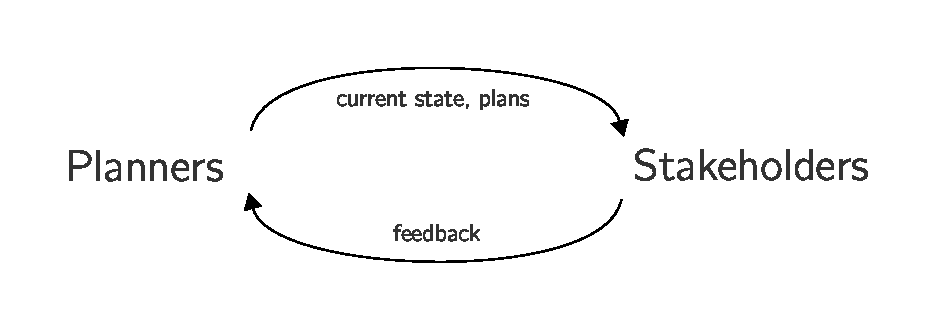
\includegraphics[width=0.7\linewidth]{figures/Loop1.pdf}
    \caption{Basic city planning loop}
    \label{fig:loop1}
\end{figure}

Looking at this loop from the stakeholders' perspective, it is in their best interest to influence the decision-making process in their favour. Similarly, local authorities should strive for more interaction between the city administration and the public. This involves making the urban data publicly available and accessible.

\section{From Data to Visualization}
As of today, the urban data is usually freely accessible in a format that is obscure for the general public. Naturally, to make the data more accessible, it is necessary to visualize it. Local authorities usually make this effort with either one of the following goals: 
\begin{itemize}
    \item to inform the public about the current state,
    \item or present the effects of a future change in the area.
\end{itemize}

Communicating the current state usually requires analysis and simplification of the raw data. There is a wide range of tools for that; however, these tools are usually proprietary, and the outputs are not that engaging. The visualization is rarely customizable; proprietary formats are used throughout the entire pipeline, and it is impossible to combine various types of data.

Communicating the future changes is even more difficult since it is required to inform the public about the current state first. In this context, the interactivity of the presentation can be the key to understanding.

We are presented with several technical challenges. The input data is often in several incompatible formats, and each describes a completely different urban domain. In other words, the datasets are often complementary, and the visualization system has to support their combination. For example, some data use different coordinate systems, or the datasets differ in their dimensionality.

If we want to create a \textit{usefull} visualization, the aforementioned technical obstacles should remain hidden from both the visualization creator and also the audience. In the ideal case, the visualization creator is given absolute freedom. The visualization system does not pose any hard restrictions on what is possible; the creator's imagination is the only limit. This utopistic idea is often contradicted by the requirement of a simple and usable interface. It is appropriate to seek a balance between unlimited possibilities and usability.

Taking into account the viewer's perspective, the goal is to make the visualization immersive enough to captivate, educate, and entertain. The physical setup and software capabilities should not diminish the experience and should avoid posing any virtual barriers between the medium and the audience.

Usually, the visualization is presented in a public space, either in museums or centers specifically equipped for this kind of presentation. While some of these places own the necessary equipment, the production pipeline today is often complicated, and an ad-hoc solution is used. In other cases, the visualization is presented using proprietary software, which is not primarily designed for the general public.

\section{The Goals}
The goal is to develop a modular system, which will streamline the urban data visualization process. The design should focus on the following four factors:
\begin{itemize}
    \item the actual communicated information,
    \item the nature of the available urban data,
    \item the creator's artistic vision,
    \item and the equipment used for the presentation.
\end{itemize}
The tricky part is that probably only one or two of those factors are known in advance --- the urban data and the used equipment can be somewhat standardized. The remaining two factors are usually project-specific; therefore, it is necessary to explore the combination of various data types and enable the freedom of artistic expression. The goal is to build a system for building other systems because of the desired modularity and adjustability --- there is an inherent metaprogramming element.